\documentclass[border=3pt]{standalone}
\usepackage{fontspec}
\IfFileExists{fonts/times.ttf}{
  \setmainfont{times.ttf}[Path=fonts/,
    BoldFont=timesbd.ttf, ItalicFont=timesi.ttf, BoldItalicFont=timesbi.ttf]
}{\usepackage{mathptmx}}
\usepackage{tikz}
\usetikzlibrary{arrows.meta,positioning,fit,backgrounds,calc,shapes.geometric}
\begin{document}
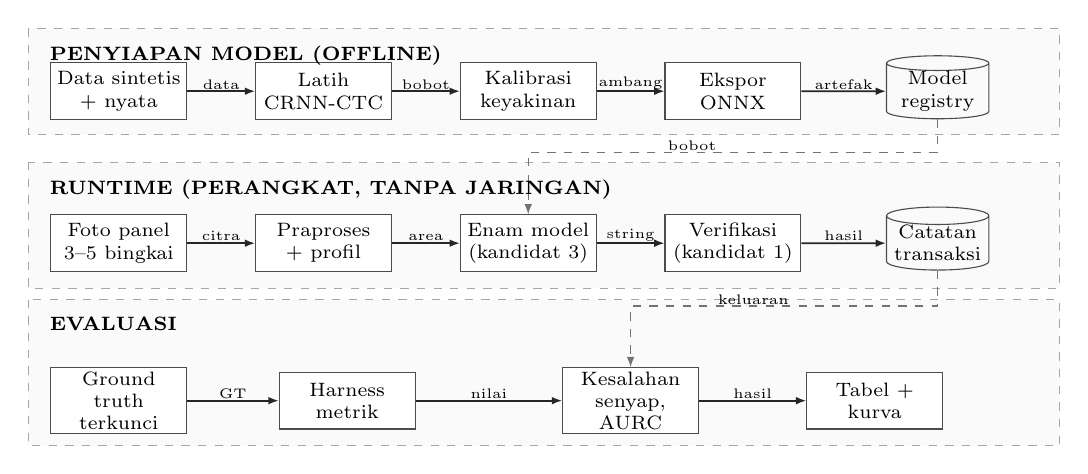
\begin{tikzpicture}[
  x=1cm, y=1cm,
  kotak/.style={rectangle, draw=black!70, fill=white, align=center,
                text width=1.62cm, minimum height=0.72cm, inner sep=1.5pt,
                font=\scriptsize},
  penyimpan/.style={cylinder, draw=black!70, shape border rotate=90,
                    aspect=0.20, minimum height=0.80cm, minimum width=1.30cm,
                    align=center, font=\scriptsize, inner sep=0pt},
  panah/.style={-{Latex[length=1.3mm]}, draw=black!85, semithick},
  panahputus/.style={-{Latex[length=1.3mm]}, draw=black!55, dashed},
  label/.style={font=\tiny, inner sep=0.5pt},
  jalur/.style={font=\scriptsize\bfseries, anchor=north west}
]

% ================= JALUR 1 =================
\node[kotak] (data)  at (1.25,0.35) {Data sintetis\\ + nyata};
\node[kotak] (latih) at (3.85,0.35) {Latih\\ CRNN-CTC};
\node[kotak] (kal)   at (6.45,0.35) {Kalibrasi\\ keyakinan};
\node[kotak] (ekspor)at (9.05,0.35) {Ekspor\\ ONNX};
\node[penyimpan] (reg) at (11.65,0.35) {Model\\ registry};

\draw[panah] (data)   -- node[label, above] {data}    (latih);
\draw[panah] (latih)  -- node[label, above] {bobot}   (kal);
\draw[panah] (kal)    -- node[label, above] {ambang}  (ekspor);
\draw[panah] (ekspor) -- node[label, above] {artefak} (reg);

% ================= JALUR 2 =================
\node[kotak] (foto)  at (1.25,-1.58) {Foto panel\\ 3--5 bingkai};
\node[kotak] (pra)   at (3.85,-1.58) {Praproses\\ + profil};
\node[kotak] (model) at (6.45,-1.58) {Enam model\\(kandidat 3)};
\node[kotak] (verif) at (9.05,-1.58) {Verifikasi\\(kandidat 1)};
\node[penyimpan] (catatan) at (11.65,-1.58) {Catatan\\ transaksi};

\draw[panah] (foto)  -- node[label, above] {citra}  (pra);
\draw[panah] (pra)   -- node[label, above] {area}   (model);
\draw[panah] (model) -- node[label, above] {string} (verif);
\draw[panah] (verif) -- node[label, above] {hasil}  (catatan);

% ================= JALUR 3 =================
\node[kotak] (gt)      at (1.25,-3.58) {Ground truth\\ terkunci};
\node[kotak] (harness) at (4.15,-3.58) {Harness\\ metrik};
\node[kotak] (metrik)  at (7.75,-3.58) {Kesalahan\\ senyap, AURC};
\node[kotak] (laporan) at (10.85,-3.58) {Tabel +\\ kurva};

\draw[panah] (gt)      -- node[label, above] {GT}    (harness);
\draw[panah] (harness) -- node[label, above] {nilai} (metrik);
\draw[panah] (metrik)  -- node[label, above] {hasil} (laporan);

% ================= KETERGANTUNGAN =================
\draw[panahputus] (reg.south) -- ++(0,-0.42) -| node[label, above, pos=0.30] {bobot} (model.north);
\draw[panahputus] (catatan.south) -- ++(0,-0.45) -| node[label, above, pos=0.30] {keluaran} (metrik.north);

% ================= KOTAK JALUR =================
\begin{scope}[on background layer]
  \draw[dashed, draw=black!35, fill=black!2] (0.10,1.15) rectangle (13.20,-0.20);
  \draw[dashed, draw=black!35, fill=black!2] (0.10,-0.55) rectangle (13.20,-2.15);
  \draw[dashed, draw=black!35, fill=black!2] (0.10,-2.30) rectangle (13.20,-4.15);
\end{scope}

\node[jalur] at (0.25,1.05) {PENYIAPAN MODEL (OFFLINE)};
\node[jalur] at (0.25,-0.65) {RUNTIME (PERANGKAT, TANPA JARINGAN)};
\node[jalur] at (0.25,-2.40) {EVALUASI};

\end{tikzpicture}
\end{document}
